%!TEX root = ../Thesis.tex

\chapter{Analysis}

\section{Background}
It is desired to develop a platform for tether control of UAV. Such a platform can have many applications in the industrial world - which also raises a number of requirements for reliability and robust design. \\
\\
The project has several issues, which needs to be addressed in the analysis in order to make a design requirement specification. This analysis will cover the issues, and the solutions will be addressed in the prototype chapter.



\section{Platform for Tether UAV}
A platform for tether control of UAV must have tree basic elements; the UAV, a power line and a Ground Station. The Ground Station supplies the power line with power and keeps track of the cable. The UAV must be able to land and take-off from the Ground Station. The power line must be light enough for the UAV to lift it. The Ground Station must assure that the power line is not touching the ground by releasing or pulling cable.

\begin{figure}[hbtp]
\centering
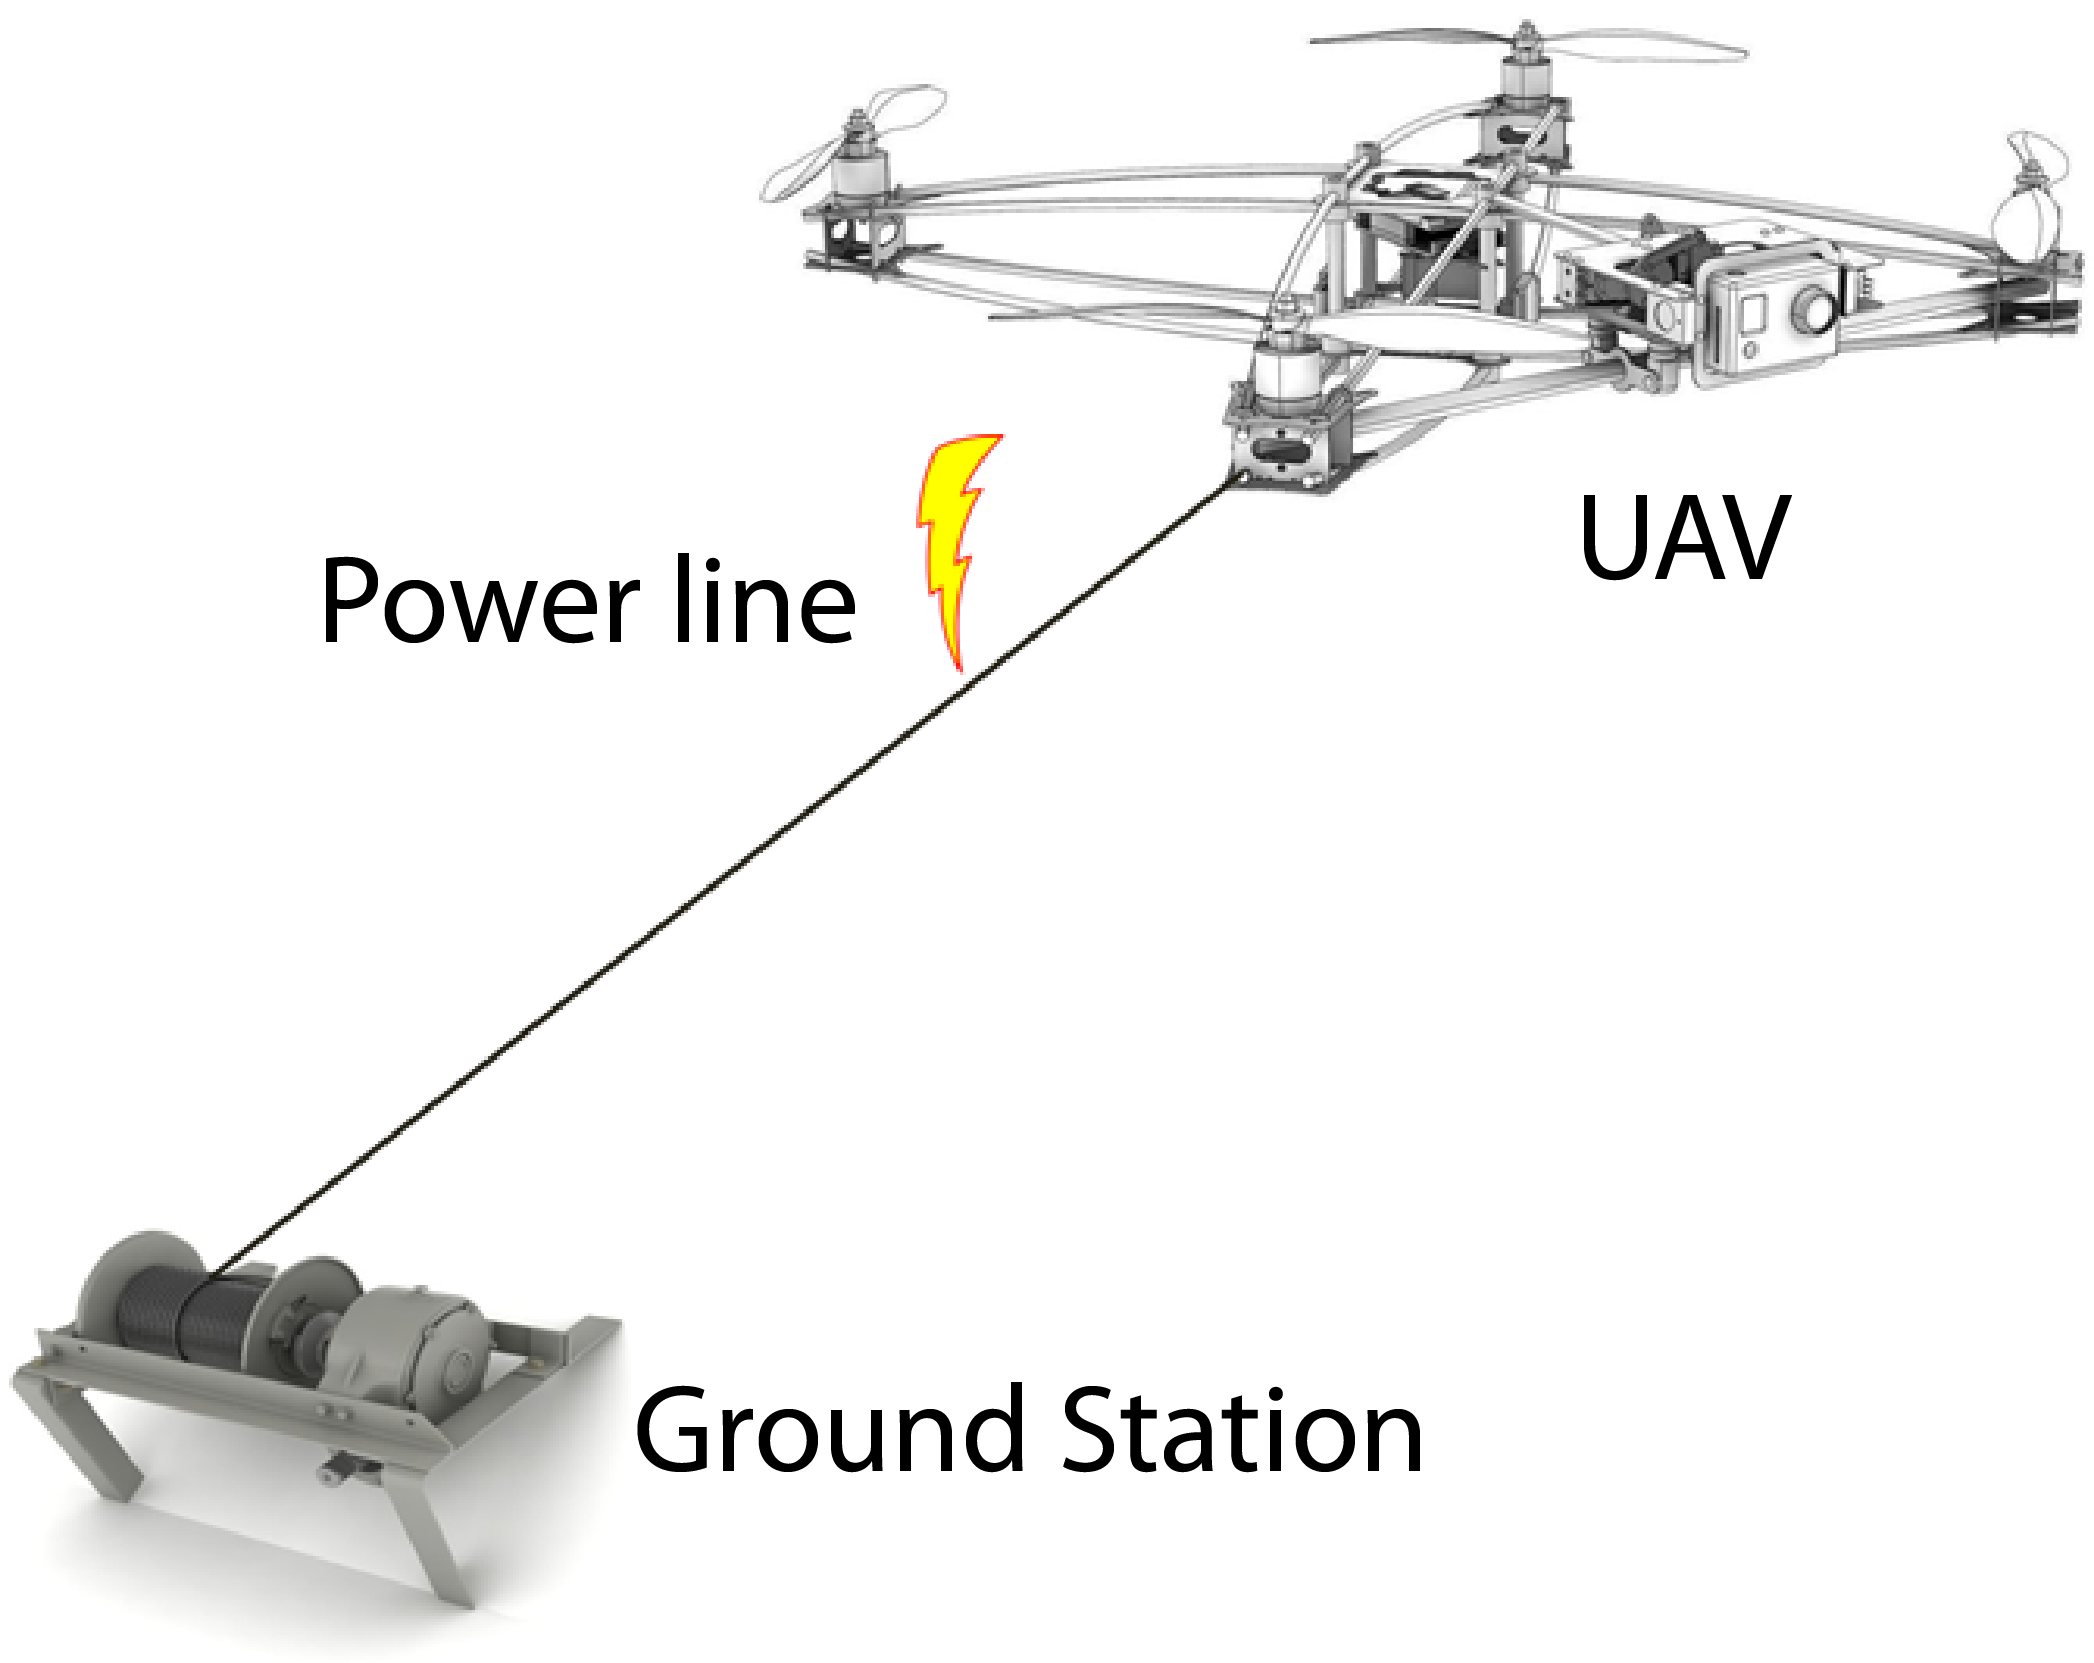
\includegraphics[scale=0.5]{graphics/overall-system.png}
\caption{Illustration of key elements for a platform for tether UAV}
\end{figure}

\section{Power line}
\noindent
Every cable has an electrical loss, and this factor contributes significantly when the cable is long and have a low cross-sectional area. Wanting to have a cable, which is as long as possible, but the UAV can only lift a limited amount of payload. The cross-sectional area and the length has a big impact on the weight. Investigating the electrical loss in the cable results in the cable specification requirements.
 
\noindent
It is assumed the UAV requires 500 watt at 12 volt when using maximal thrust\cite{Wahlgreen2014}. To be on the safe side adding a tolerance of 10 per cent, ending up with supplying the UAV with 550 watt. 
Calculating the cable loss as following. 
$P$ is the power in Watt, $U$ is the voltage in Volt, $l$ is the cable length in meter, $\rho$ is the electrical resistivity in $\Omega \cdot m$ and $A$ is the cross sectional area in $m^2$.
\noindent
The current $I$, in ampere, through the wires is given by the power divided with the voltage.
\begin{equation}
I = P/U \quad [\mathrm{A}]
\end{equation}
\noindent
The resistance $R$, in ohm, per unit length is to be determined by the electrical resistivity $\rho [\Omega \cdot m]$ divided by the conductors cross sectional area, $A$.

\begin{equation}
R = \frac{\rho}{A}\quad [\Omega]
\end{equation}
\noindent
The voltage drop $U_{drop}$ per unit length is to be determined by the current times the resistance.

\begin{equation}
U_{drop} = I \cdot R \quad [V]
\end{equation}
\noindent
The voltage drop depends on the current going through the wire and the resistance. It is favourably to have a high voltage and low current to minimize the voltage drop; hence, the voltage drop is independent of the voltage. It is a commonly known method used in power supply systems all over the world. For a low voltage, the per cent of voltage drop is very high, as illustrated on figure \ref{fig:relation_voltage_drop}.

\begin{figure}[hbtp]
\centering
\includegraphics[scale=1]{graphics/matlab/cable_relation_voltage_drop.eps}
\caption[Relationship between voltage drop and cable length per ampere]{Relationship between voltage drop and cable length per ampere over a 50m cable. A is the cross-sectional area of the conductor.}
\label{fig:relation_voltage_drop}
\end{figure}

\noindent
In order to avoid the Low Voltage Directive \cite{Parliament2006} the DC voltage must be less or equal to 75 volt. 75 volt DC is easily achieved with standard components and therefore set as the power transmission voltage. \\

\noindent
The cable loss $P_{loss}$, in Watt, per unit length is now given by
\begin{equation}
P_{loss} = I^2 \cdot R \quad [\mathrm{W}]
\end{equation}
\noindent
The loss in the cable needs to be minimal. A known method to minimize the loss on the cable is to step up the voltage. This is because of the fact the loss depends on the current squared times resistivity and independent of the voltage. 


\begin{figure}[hbtp]
\centering
\includegraphics[scale=1]{graphics/matlab/cable_relation_lenght_loss_crosssection.eps}
\caption[Relationship between cable length, cross-sectional area and cable loss.]{Relationship between cable length, cross-sectional area, and  loss.}
% Calculated with copper resistivity and for both + and GND conductor cores.
\label{fig:relationship_loss_length}
\end{figure}


\noindent
On figure \ref{fig:relationship_loss_length} it is seen the electrical loss in the conductor also depends on length and cross-sectional area of the conductor. The electrical loss is converted into heat in the cable.

\newpage
\section{Tension force in the Cable}

\noindent
In a simplified model, the weight of the cable will only drag the UAV on one axis, towards the Ground Station. On the UAV there is one load cell mounted, measuring the force in the direction of the tension. The output of the load cell will enable the Ground Station to decide if it should roll cable out or in. However, this simplified model assumes the UAV perpendicular to the cable at all times. 
In the real world, this is only true when it hovers directly over the Ground Station. As the UAV goes to one of the sides, it will try to maintain horizontal pitch/tilt. The cable will try to drag the UAV in the direction of the Ground Station, cause at steady force the UAV have to work against. Because of aerodynamics the UAV will tilt in some extend to work against the tension. If this tilt get to large, the UAV will lose its lifting capability, therefore stall, and crash towards the ground.


   

\subsection{Modelling the Tension in the Free Hanging Cable}
Modelling the cable in the real world has a great complexity and in order to make a robust design we must assume the surrounds are not ideal. The ideal case is the cable is hanging in a direct line, as seen on figure \ref{fig:cable_model_cases}. Only at the anchor point, the cable touches the ground. Worst-case scenario is all cable is lying on the ground, except what is directly underneath the UAV. Assuming the cable will be in between the direct line and worst case. The maximal position error will be the difference between the direct line and worst-case line, calculated to approximately $14.65$ meters or 29.3 per cent.

\newpage

\begin{figure}[H]
\centering
\includegraphics[scale=1]{graphics/matlab/cable_arc_approx.eps}
\caption[Diagram showing four ways of approximate the cables position.]{Diagram showing four ways to approximate the cables position. The direct line is the ideal case. The area between the ideal and worst case is the actual working area where it has assumed the position of the UAV to be. Position estimation using a circular shape and catenary chain to approximate the position.}
\label{fig:cable_model_cases}
\end{figure}

\noindent
Both the direct line and worst case is possible, but highly unlikely in the real world. A cable hanging between two points will have a curved shape from the sag and the cable flexibility. Assuming the curve from the sag is described as a circle, the cable will curve uniformly over the entire length. This assumes the cable has no mass, but in the real world, it has.
The catenary chain is close to a parabolic shape but describes the curve of a freely hanging chain with the mass uniformly distributed\cite{Whewelll1833}. The catenary equation have the form:

\begin{equation}
y = a \cdot \cosh\left(\frac{x}{a}\right)
\end{equation}
The catenary chain assumes the cable is so flexible that any force exerted by the chain is parallel to the chain. This set a requirement for the bending radius for the cable to be much less than the length of the cable.
The weight of the cable pulls the UAV down and towards the anchor point. Let the point $c$ be the anchor point to the ground and $r$ be a force vector at the anchor point on the UAV. $r$ must be at a higher point than $c$. The force $T_0$ at point $c$ is tangential to the curvature thus only has a $x$ component. The force $T$ at point $r$ is tangential to the curvature at point $r$ and can be described as
\begin{equation}
T = T \cos(\phi) +  T\sin(\phi)
\end{equation} 
$\phi$ is the angle between the $x$ axis and the force vector and $T$ is the magnitude of the force. The cable weight is represented as $\lambda$ per unit length. $g$ is the gravitational force and $s$ is the length of the cable. The downward force is therefore $-\lambda g s$.

\begin{figure}[hbtp]
\centering
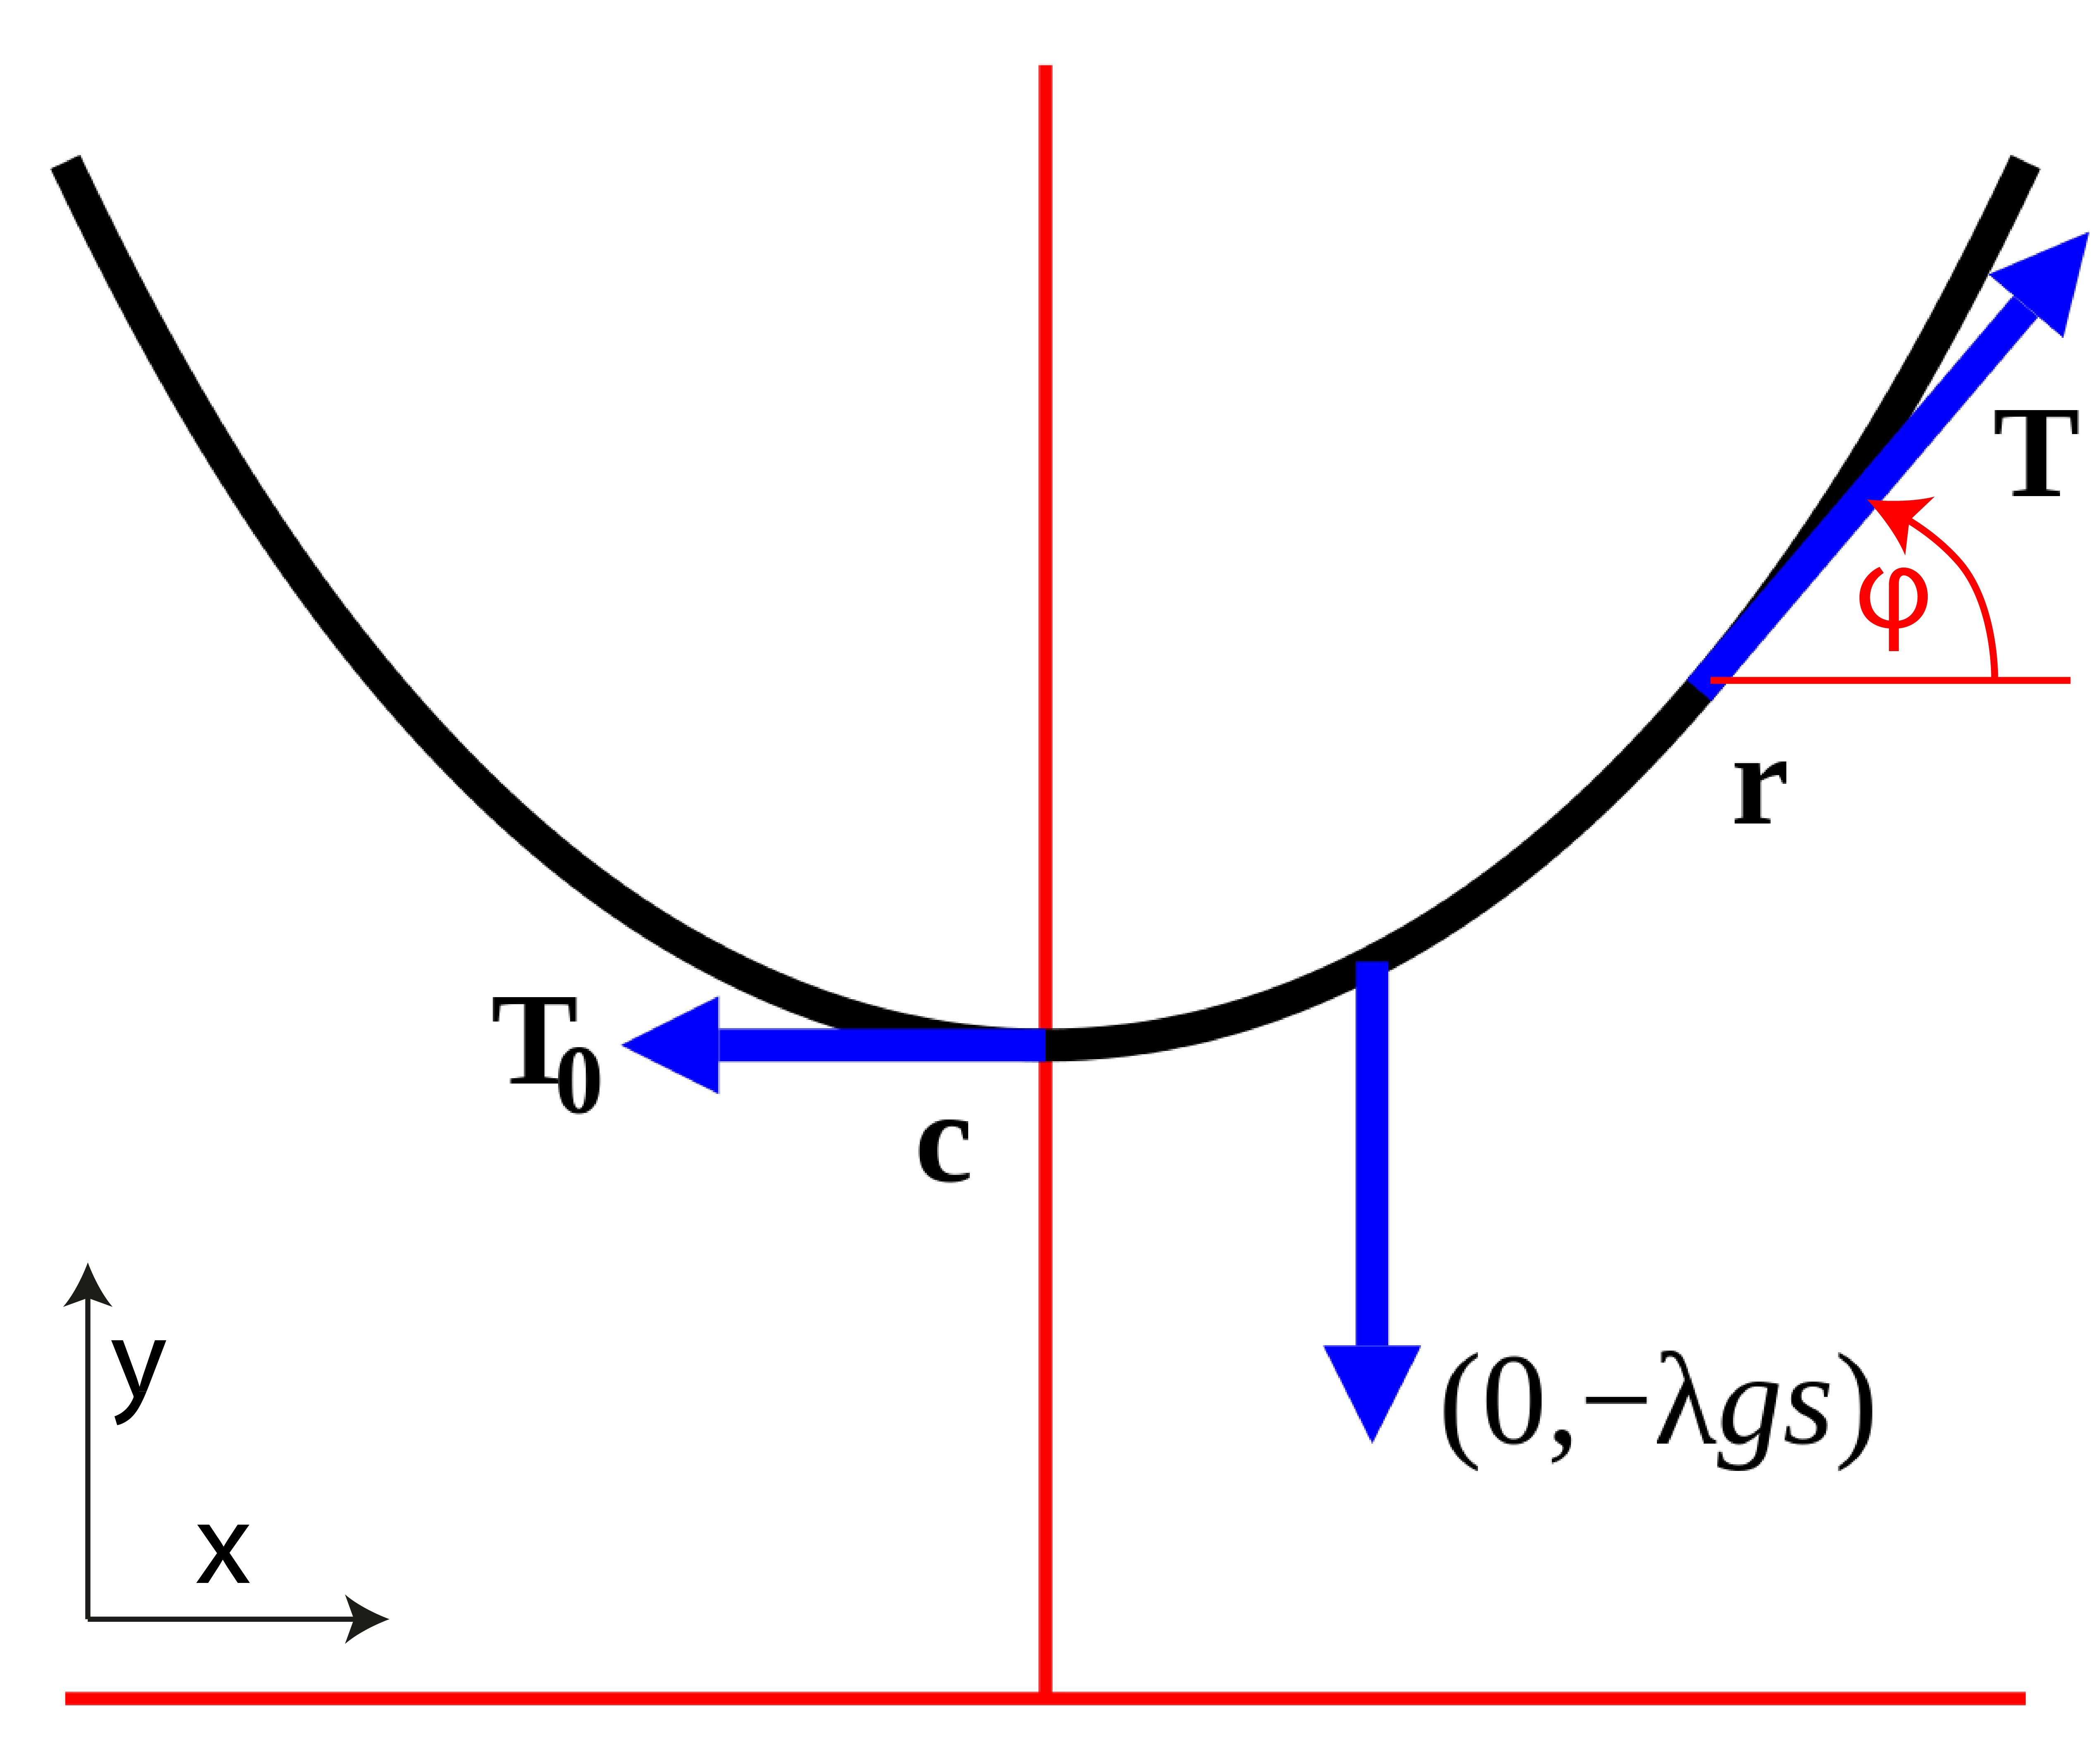
\includegraphics[scale=0.25]{graphics/CatenaryForceDiagram.png}
\caption[Catenary Chain Force diagram]{Catenary Chain Force diagram displaying forces acting from anchor point $c$ to point $r$. $T_0$ is the tension at anchor point $c$ and $T$ is the tension at point $r$. Note the $y$ axis in this diagram will correspond to the height later denoted as $z$ in a tree dimensional coordinate system.}
\label{fig:catenary_force_diagram}
\end{figure}

\noindent
In this analysis the cable is in equilibrium thus the sum of the tree forces is zero. 
\begin{equation}
\sum T_0 + T -\lambda gs = 0
\end{equation}
Splitting up the sum in $x$ and $y$ components gives:
\begin{eqnarray}
T\cos(\phi) =& T_0 \\
T \sin(\phi) =& \lambda g s
\end{eqnarray}
Resulting in the expected force at $T$ as a function of either the force at the anchor point or the cable length, and $\phi$.
\begin{equation}
T = \frac{T_0}{\cos(\phi)} = \frac{\lambda g s}{\sin(\phi)}
\end{equation}

\noindent
To be able to model the cable using the catenary chain four parameters must be available; the tension at anchor point $T_0$, the angle at the UAV $\phi$, the total force at the UAV, and the length of the cable.\\

\noindent
This model excludes all cases where either the UAV is below the anchor point or the cable fully or partially is below the anchor point.



   

\subsubsection{Horizontal Angular Force Measurement}
\label{sec:horizontalMeasurementAnalysis}
\begin{figure}[hbtp]
\centering
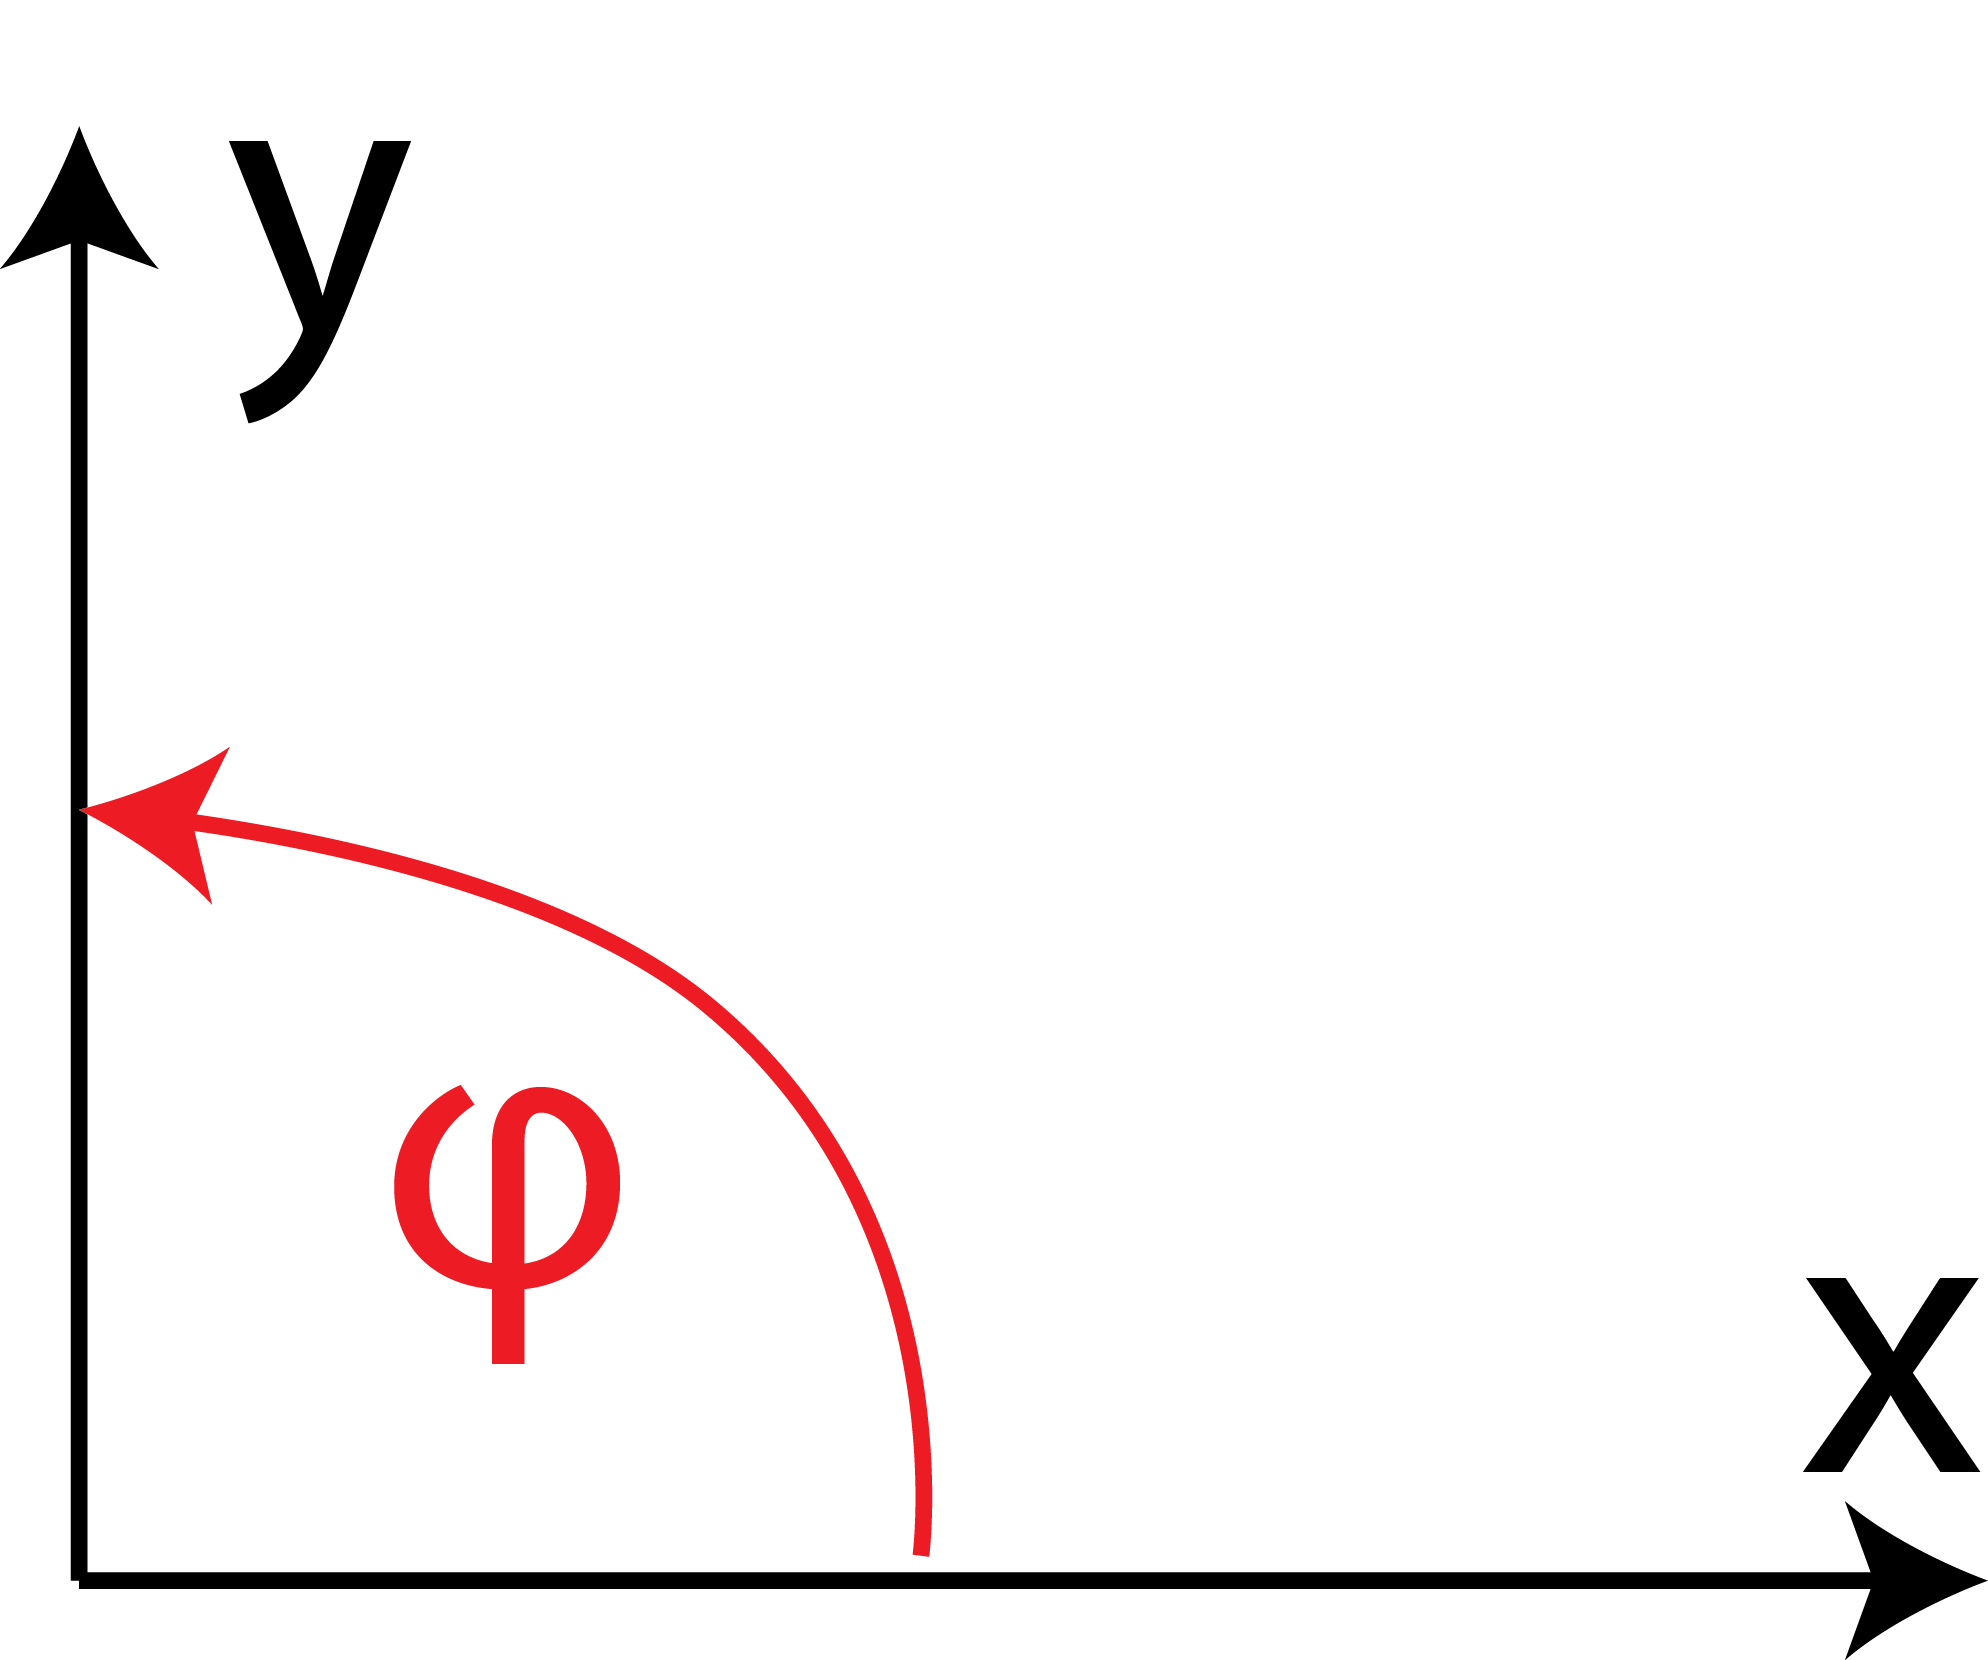
\includegraphics[scale=0.25]{graphics/horizontal_coordinatesystem.png}
\caption{Coordinate system for horizontal measurement device.}
\end{figure}

\noindent
Measuring the horizontal angle, $\phi$, relative to the Ground Control Station and the UAV; a 2-axes measuring device is needed. The two axes must be perpendicular to each other. In that way a scalar of two unit vectors $\hat{x}$ and $\hat{y}$ can represent the tension from the cable in a combination of each direction. 
From the length of the scaled vectors $\overline{X}$ and $\overline{Y}$ the angle $\phi$ can be found.

\begin{equation}
\phi = \mathrm{atan2} (Y,  X) = 2 \cdot \mathrm{arctan} \frac{\sqrt{X^2+Y^2}-X}{Y}
\end{equation}

\noindent
$\phi$ is the angle from the positive $\hat{x}$-direction and increases counter clockwise. 

\noindent
The length of $\overline{XY}$ is given by:
\begin{equation}
\overline{XY} = \sqrt{X^2+Y^2}
\end{equation}

\noindent
The length og $\overline{XY}$ corresponds to the $T_0$ tension in the cable in $\phi$ direction. 

\subsubsection{Tree Dimensional Force Measurement at the UAV}
The UAV has tree degrees of freedom in space, thus a tree axes measurement devices is needed in order to measure the total force $T$.  The measurement device must measure the force relative to the UAV, thus if the UAV tilted to one side, by roll or pitch, it will not be adjusted in the angular calculation of $\theta$.  


\begin{figure}[hbtp]
\centering
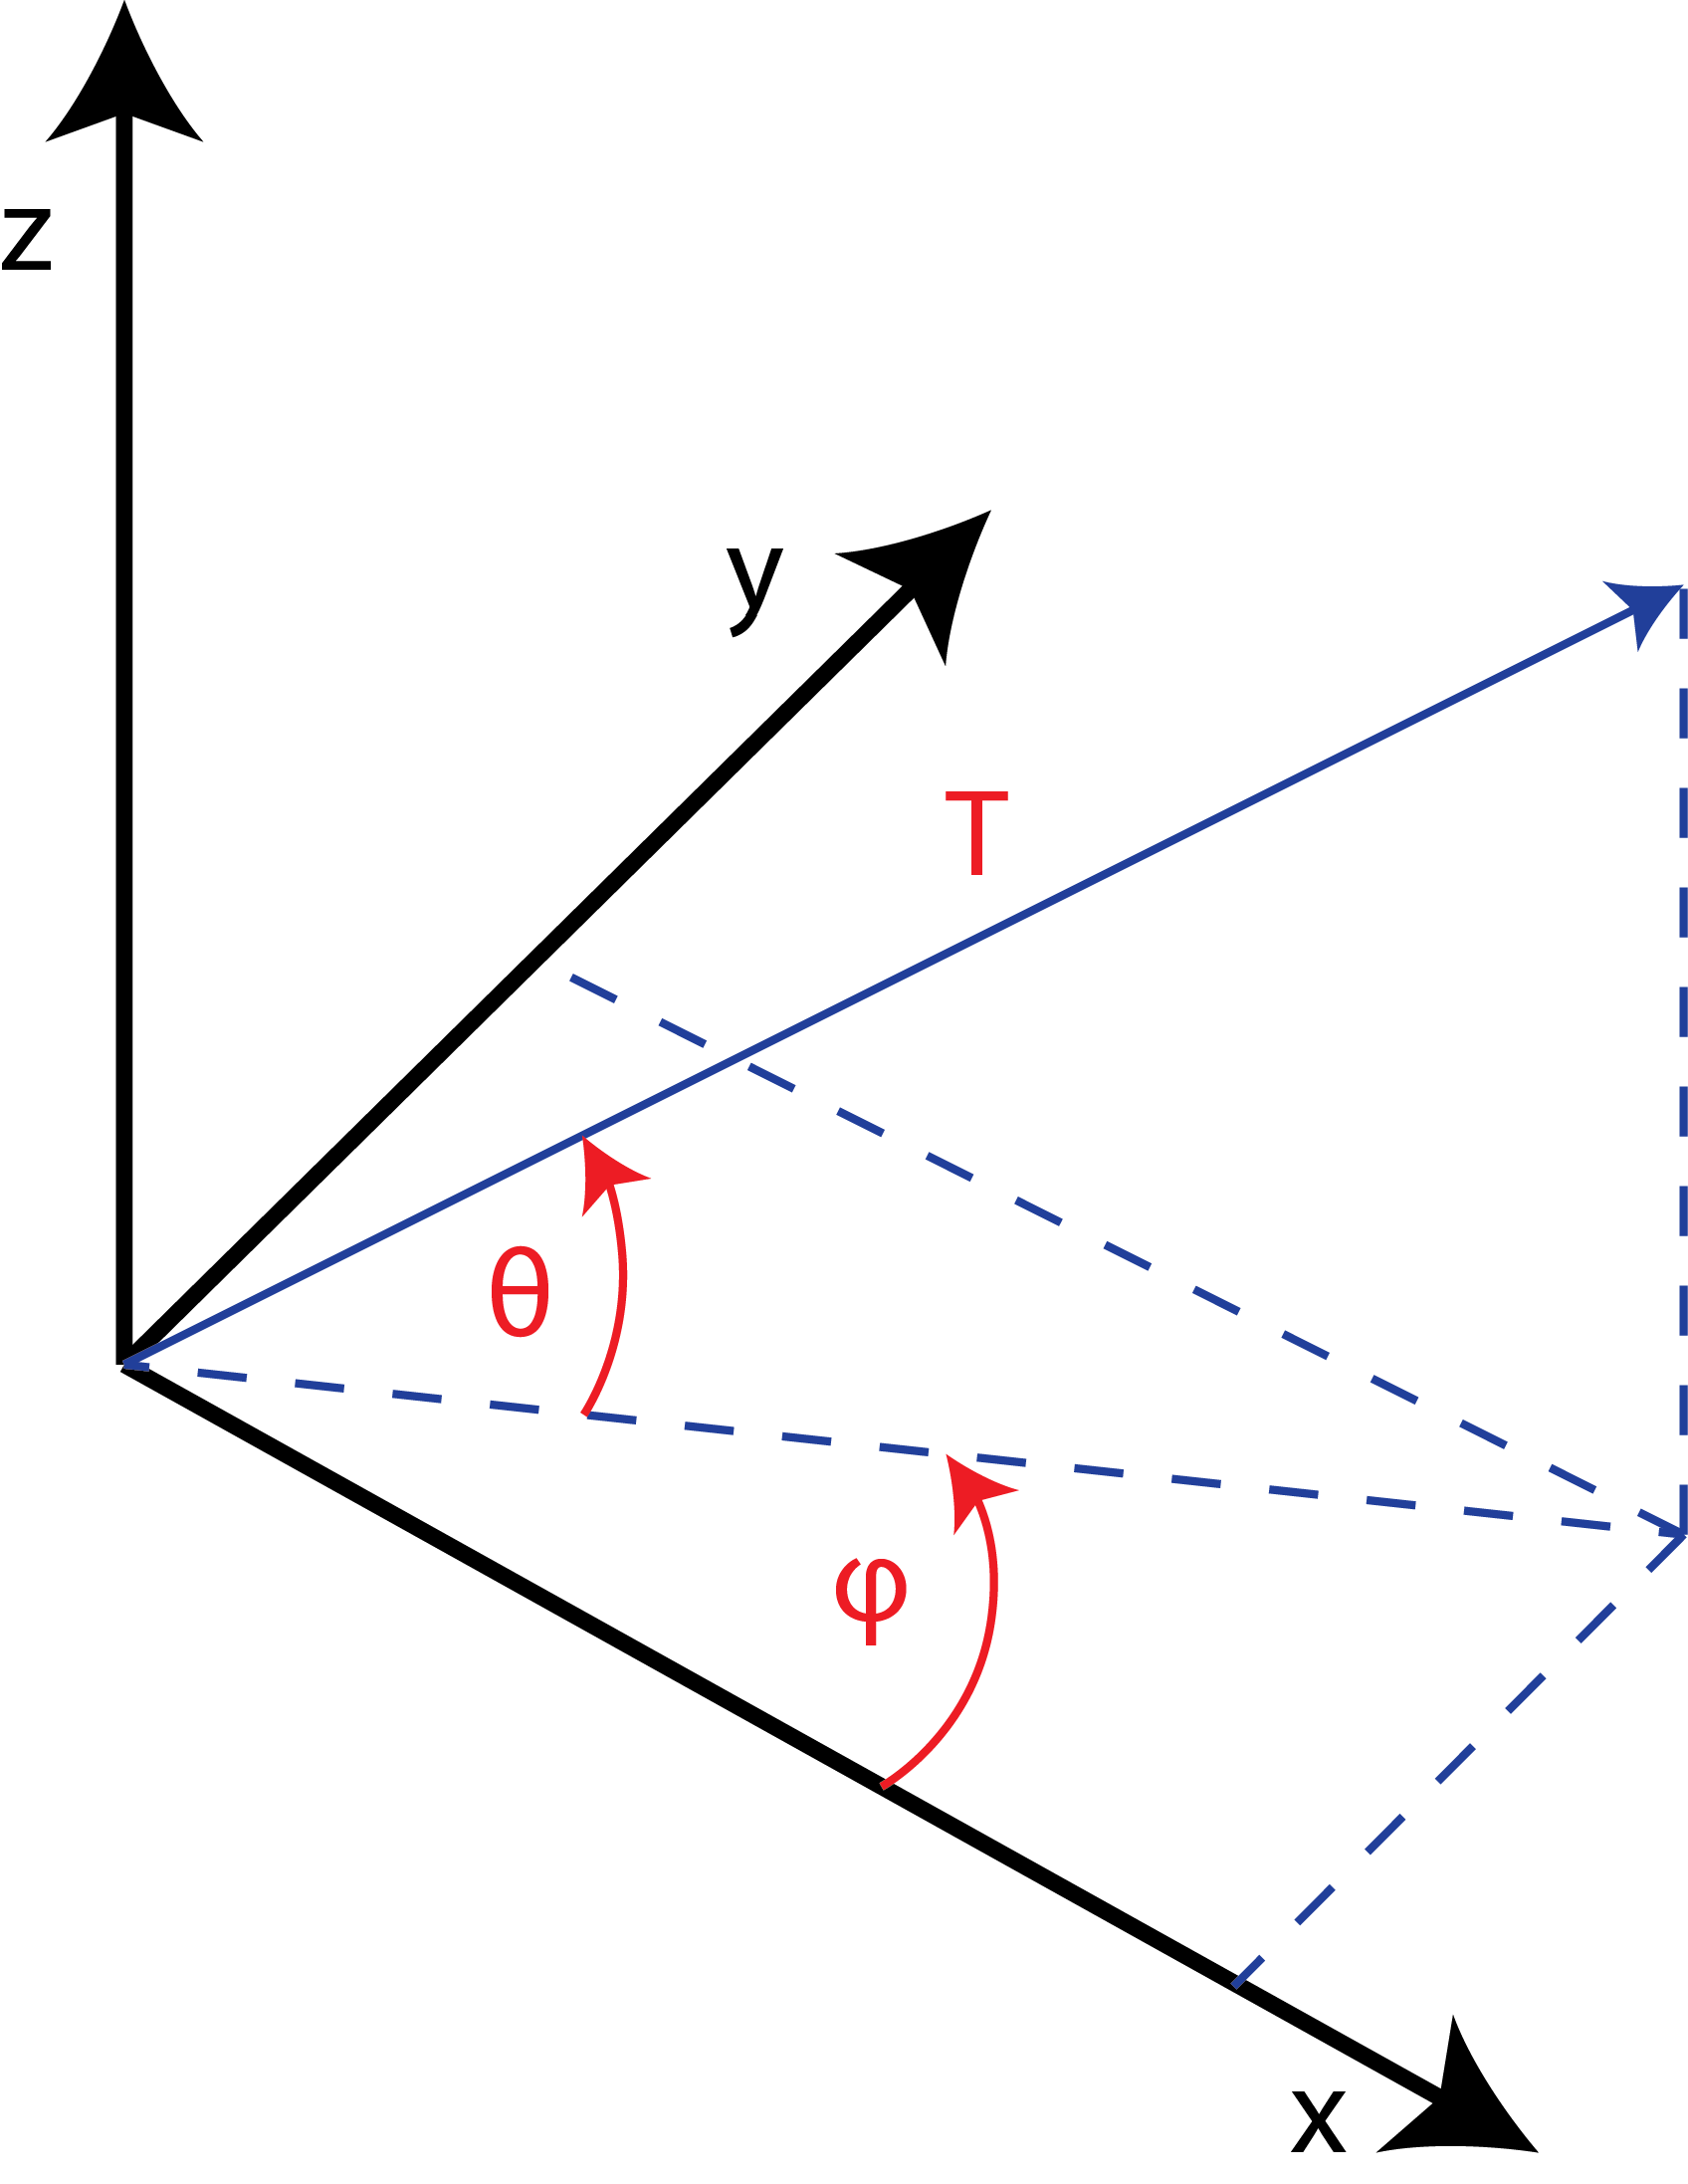
\includegraphics[scale=0.5]{graphics/UAV-force-diagram.png}
\caption[Force diagram for UAV]{Diagram showing the force $T$ the UAV have to withstand from the cable.}
\end{figure}

\noindent
Calculating the total force from the tree axes using the same method as in the Horizontal Measurement Device.

\begin{equation}
T = \sqrt{x^2+y^2+z^2}
\end{equation} 

\noindent
To determine the direction of the total force the angle between $x$- and $y$-axes is denoted as $\phi$ and the angle between the $xy$-plane and $z$-axis is denoted as $\theta$.
$\phi$ is derived as in the horizontal force measurement device.
\begin{equation}
\phi = \mathrm{atan2}(y,x)
\end{equation}

\noindent
$\theta$ is derived as the inverse cosine to the force in the $z$-direction over the total force.
\begin{equation}
\theta = \mathrm{acos}\left( \frac{z}{T} \right)
\end{equation}

\subsection{Load cell}
The load cells used in this project is a single-point load cell. Determining the type and brand of load cells based on the availability/flexibility to create multidimensional measurements and the cost. A load cell is a strain gauge (flexibly resistor pattern) that will change resistance when bended, mounted on a flexible material. In this case, a block is cut out of Aluminium and a strain gauge is mounted on one surface. When the aluminium is exerted with a force or weight, it will bend slightly, causing a small change of resistance in the strain gauge. The change of resistance can be measured by a Wheatstone bridge, as the one on the Phidget bridge\footnote{Phidget bridge 1046, http://www.phidgets.com/products.php?product\_id=1046}.

\noindent
The calibration of the load cell is very important to obtain a useful reading. The calibration converts the measured value to the measured force.  
\begin{eqnarray}
F =& K_f \cdot (V_{in} - b)\\
W =& K_w \cdot (V_{in} - b)
\end{eqnarray}
$F$ and $W$ is the expected force and weight. $K$ is a gain value depending on whether the output unit is force or weight. The offset $b$ will vary between individual load cell, even from the same batch. $V_{in}$ is the value reading from the Phidget bridge. The size $V_{in}$ depends on the gain set in the Phidget configuration.\\
\noindent
When dealing with multiple load cells there are two ways of configuring them electrical wise. First is to measure each load cell individual and second to measure all together. The first one has the advantage of being able to measure each load cell individually, but the disadvantage of using many inputs and each load cell needs to be calibrated individually. Second, one has the advantage of only using one input on the bridge and all cells can be calibrated together, but the disadvantage of all load cells need to be of same type and size and not being able to measure each load cell individually. In this project, the information of direction of the tension is important and because of that measuring each load cell individually is the best solution\cite{PhidgetsInc.2012}.

\subsection{Data Connection}
The measurements from both the Ground Station and the UAV is used as position references in the position controller on the UAV. Thus, the data sent to the PixHawk flight controller must have as little delay as possible.

\newpage
\section{Design Requirement Specification}
\begin{itemize}
\item The UAV must be capable to stay airborne significantly longer time than a battery powered alternative.
\item Supply the UAV with 12 volt DC and 500 watt.
\item The weight of the cable must not be greater than the lifting capability of approximately 3kg \cite{Sidea2013}.
\item The system must not be subject to the Electrical Safety: Low Voltage Directive, and therefore keep any voltage under 75 volt DC \cite{Parliament2006}.
\item Given the cheap cost of UAVs today, the solution must keep a low material cost.
\item Measuring the total horizontal force at the anchor point.
\item Measuring the total force and direction at the UAV.
\item Measuring the length of the free hanging cable.
\item The Ground Station is supplied with 12 volt.
\end{itemize}





